\documentclass[final]{beamer}
\usepackage[size=a0,scale=1.2]{beamerposter} % tamaño A0, puedes cambiarlo a a1, a2...

%-----------------------------------------------------------
% Paquetes útiles
%-----------------------------------------------------------
\usepackage{graphicx}   % Para incluir figuras
\usepackage{amsmath,amssymb}
\usepackage{qrcode}     % Para generar código QR
\usepackage{multicol}
\usepackage{booktabs}   % Para tablas bonitas

%-----------------------------------------------------------
% Datos del cartel
%-----------------------------------------------------------
\title{Explorando sistemas cuánticos con Python: una guía para el salón de clases}
\author{Tu Nombre, Asesor: Dr. XXX}
\institute{Universidad de Sonora}
\date{Congreso Nacional de Física, 2025}

%-----------------------------------------------------------
\begin{document}
\begin{frame}[t]

%-----------------------------------------------------------
% Estructura en 3 columnas
%-----------------------------------------------------------
\begin{columns}[t,totalwidth=\textwidth]

%===========================================================
% Columna 1
%===========================================================
\begin{column}{0.32\textwidth}
  \begin{block}{Introducción y Motivación}
    \begin{itemize}
      \item Métodos computacionales enriquecen la enseñanza de mecánica cuántica.
      \item Python permite implementar algoritmos accesibles para estudiantes.
      \item Este trabajo presenta dos niveles:
      \begin{enumerate}
        \item Método de Numerov (oscilador armónico y átomo de hidrógeno).
        \item Método de Hartree–Fock (moléculas diatómicas).
      \end{enumerate}
    \end{itemize}
  \end{block}

  \begin{block}{Metodología}
    \textbf{Numerov:}
    \begin{itemize}
      \item Integración eficiente de la ecuación de Schrödinger 1D.
      \item Aplicación: autofunciones del oscilador armónico, estados radiales de H.
    \end{itemize}
    \vspace{1em}
    \textbf{Hartree–Fock:}
    \begin{itemize}
      \item Aproximación autoconsistente para moléculas.
      \item Aplicación: H$_2$, HeH$^+$.
    \end{itemize}
  \end{block}
\end{column}

%===========================================================
% Columna 2
%===========================================================
\begin{column}{0.32\textwidth}
  \begin{block}{Resultados: Numerov}
    \begin{center}
      % Pon aquí tus gráficas del oscilador y del H
      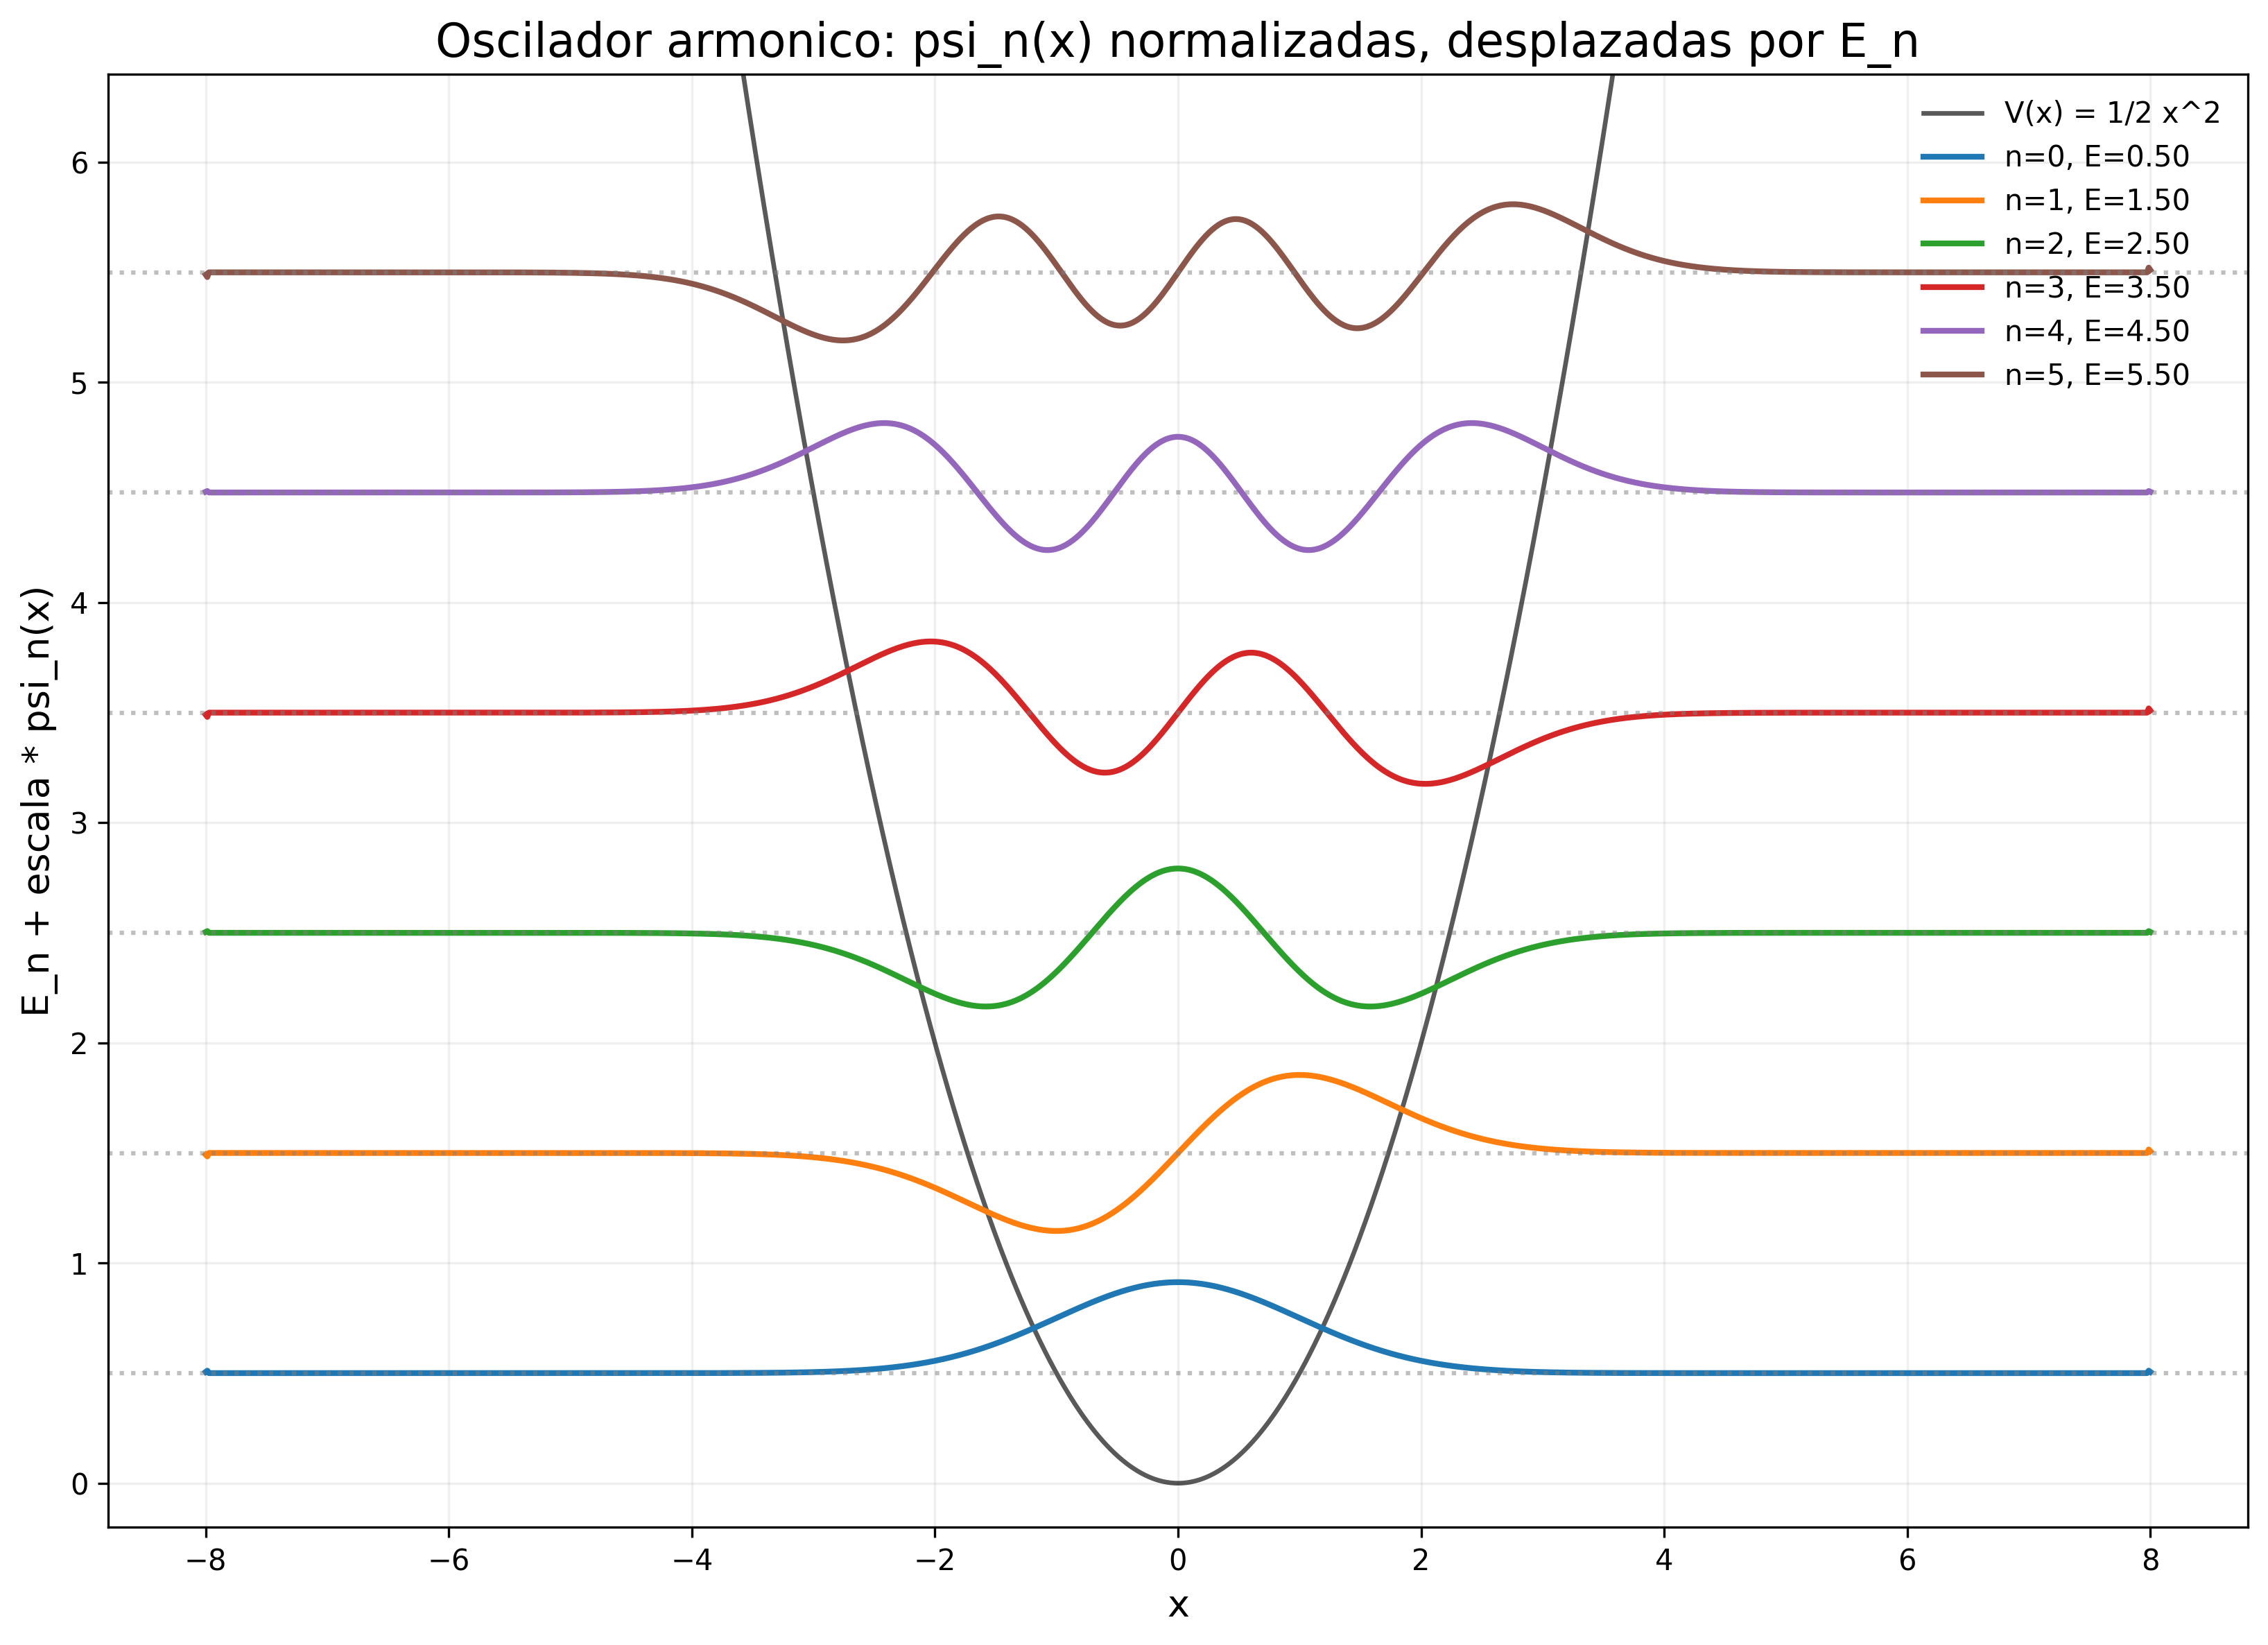
\includegraphics[width=0.95\linewidth]{harmonic.png}\\
      \vspace{0.5cm}
      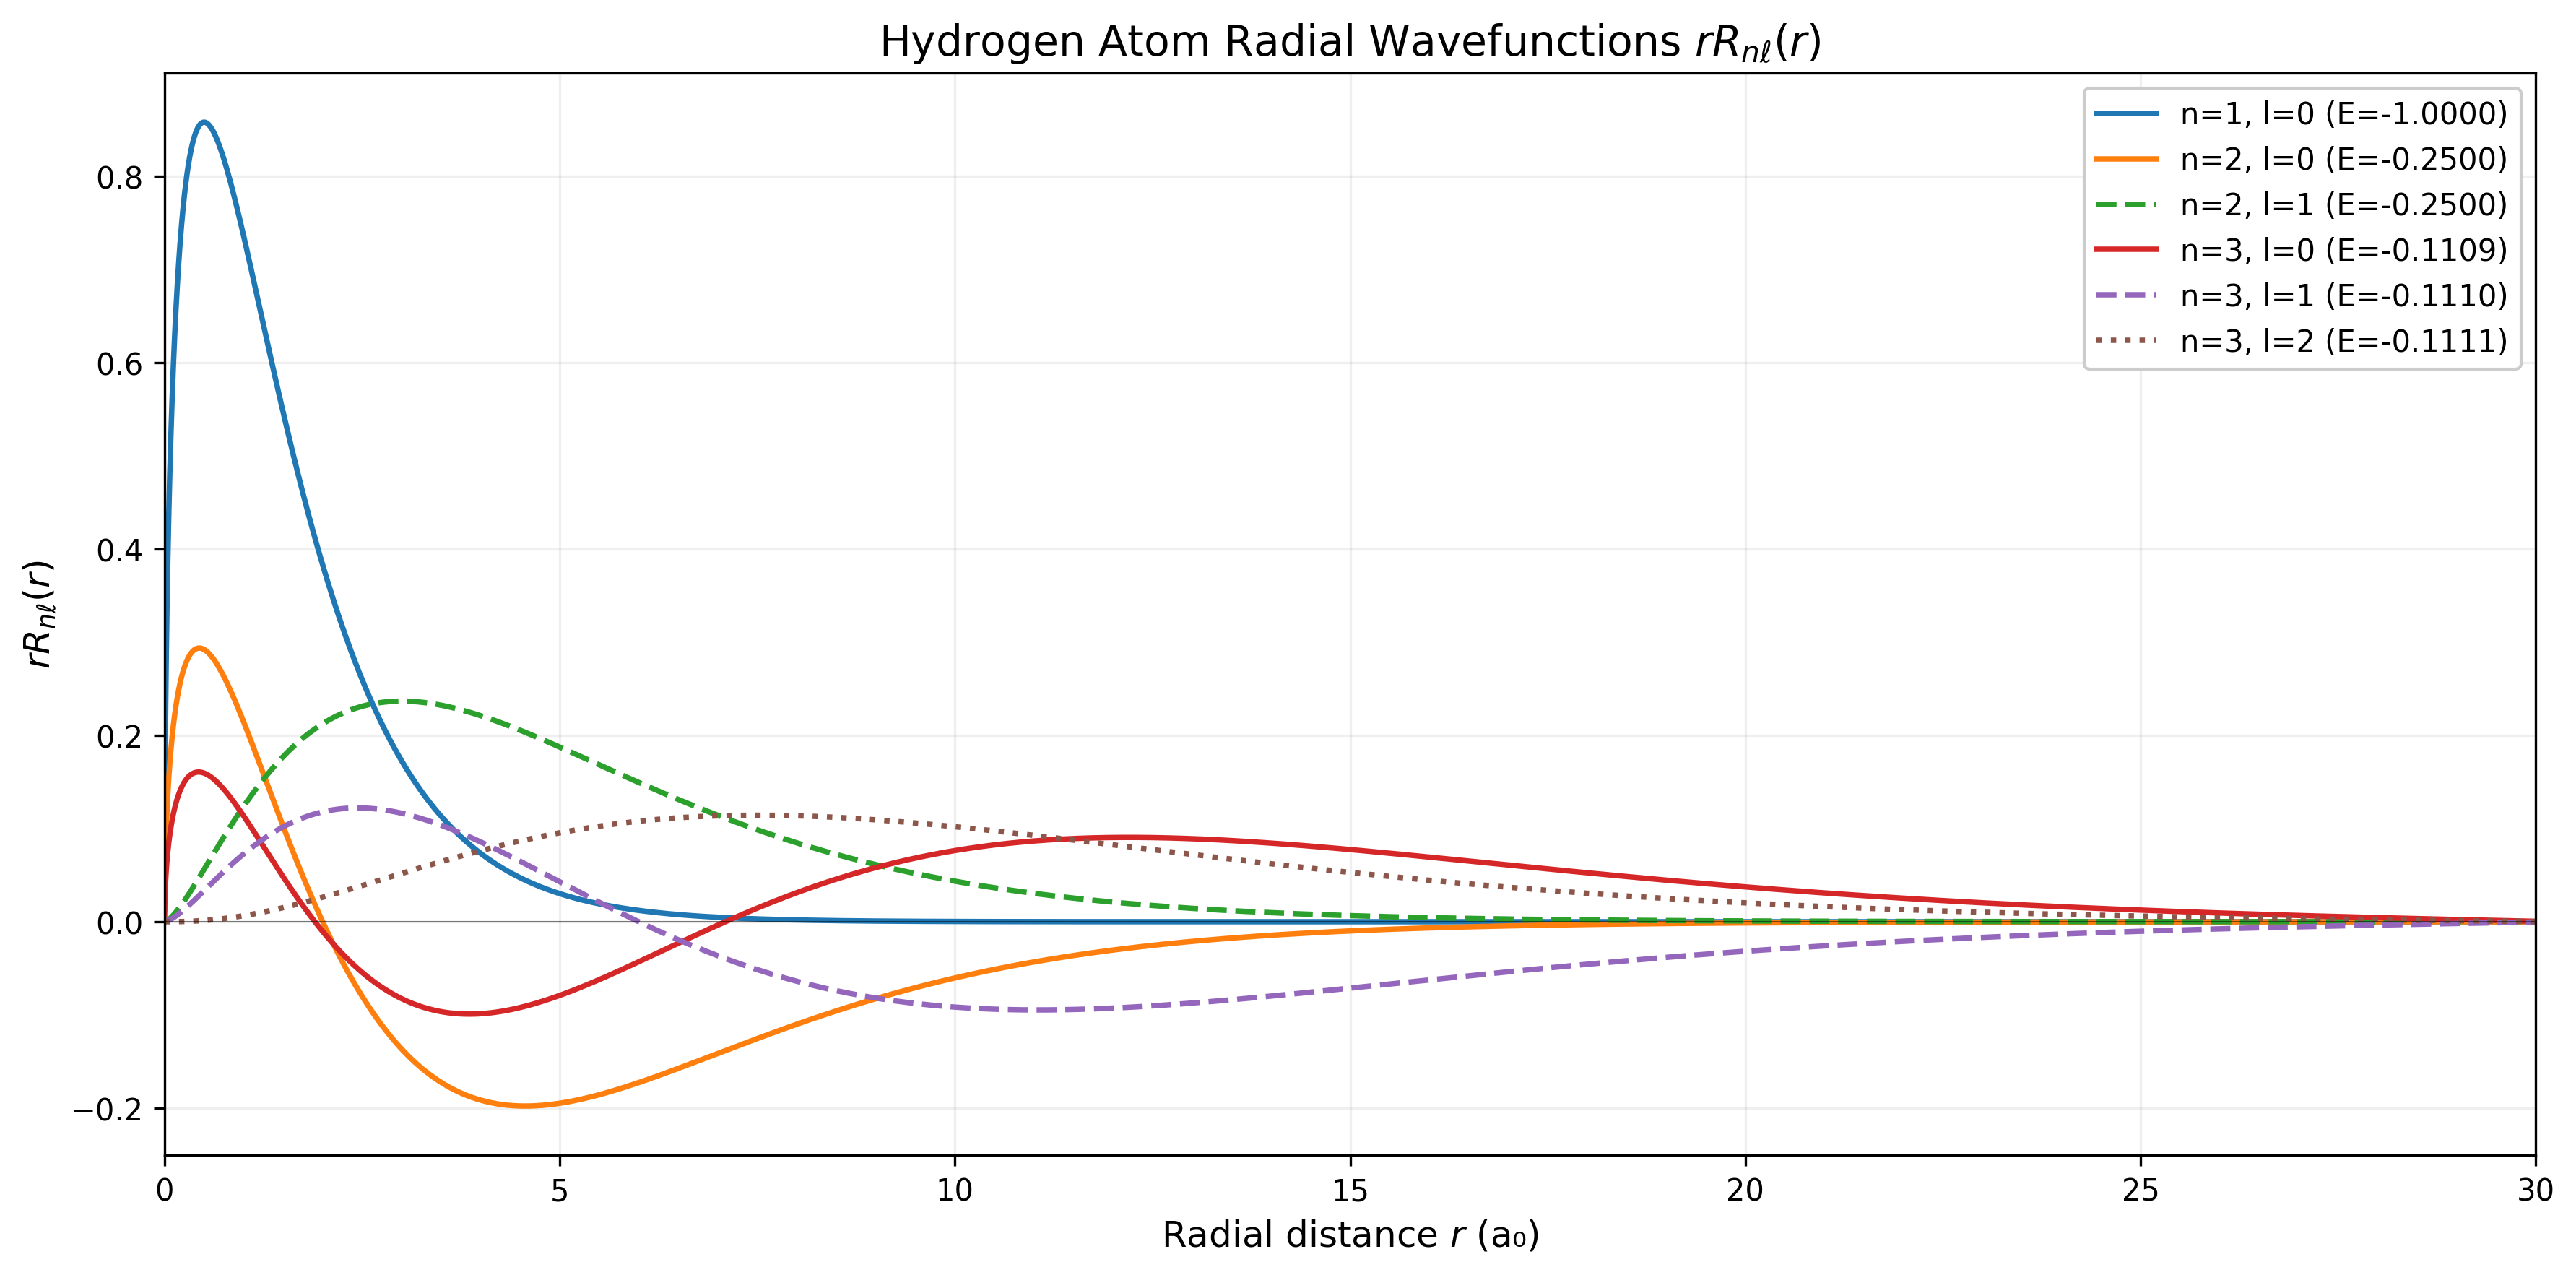
\includegraphics[width=0.95\linewidth]{hydrogen.png}
    \end{center}
  \end{block}

  \begin{block}{Resultados: Hartree–Fock}
    \begin{center}
      % Pon aquí curvas de energía para H2 y HeH+
      \includegraphics[width=0.95\linewidth]{H2.png}\\
      \vspace{0.5cm}
      \includegraphics[width=0.95\linewidth]{HeH+.png}
    \end{center}
  \end{block}
\end{column}

%===========================================================
% Columna 3
%===========================================================
\begin{column}{0.32\textwidth}
  \begin{block}{Aplicación Didáctica}
    \begin{tabular}{@{}ll@{}}
      \toprule
      Curso & Método \\
      \midrule
      Intro Mecánica Cuántica & Numerov (oscilador, H) \\
      Física Cuántica & Hartree–Fock (H$_2$, HeH$^+$) \\
      \bottomrule
    \end{tabular}

    \vspace{1em}
    \textbf{Taxonomía de Bloom:}
    \begin{itemize}
      \item \textit{Comprender}: Plantear la ecuación de Schrödinger.
      \item \textit{Aplicar}: Usar Numerov en casos simples.
      \item \textit{Analizar}: Comparar resultados numéricos con soluciones analíticas.
      \item \textit{Evaluar/Crear}: Extender Hartree–Fock a nuevos sistemas.
    \end{itemize}
  \end{block}

  \begin{block}{Conclusiones}
    \begin{itemize}
      \item Python facilita experiencias prácticas de alto nivel en licenciatura.
      \item Numerov y Hartree–Fock conectan teoría y aplicación.
      \item El material apoya al docente en cursos saturados de contenido.
    \end{itemize}
  \end{block}

  \begin{block}{Repositorio}
    Escanea el código QR para acceder al material completo y al código:
    \begin{center}
      \qrcode{https://github.com/recore799/schrodinger1d}
    \end{center}
  \end{block}
\end{column}

\end{columns}
\end{frame}
\end{document}
